\documentclass{beamer}
\usepackage{multirow}
\usepackage{tabularx}
\usepackage{kotex}
\usepackage{amsmath}
\usepackage{amssymb}
\usepackage{graphicx}
\usepackage{caption}
\usepackage[backend=bibtex, style=authortitle-comp]{biblatex}
\addbibresource{references.bib}

\usetheme{Boadilla}
\title[NFG-VAE]{Learning semi-Markovian DAGs with flow-based VAE}
\author[Seoul National University]{Dangchan Kim, Byungguk Kang, Jaeseok Kim, Minchan Kim}
\institute[]{Seoul National University}
\date{\today}

\renewcommand{\footnotesize}{\fontsize{7pt}{5pt}\selectfont}

\begin{document}

\frame{\titlepage}

\setbeamertemplate{section in toc}[ball unnumbered]
\begin{frame}
    \frametitle{Table of Contents}
    \tableofcontents
\end{frame}

% This beamer tex file is based on my paper.tex

\section*{Overview}

\begin{frame}{Overview}
    \begin{itemize}
        \item \textbf{Problem}: Learning semi-Markovian DAGs
        \item \textbf{Solution}: Normalizing flow based VAE
        \item \textbf{Contribution}
        \begin{itemize}
            \item A new method for learning semi-Markovian DAGs
            \item A new method for learning DAGs with non-Gaussian noise
        \end{itemize}
    \end{itemize}
\end{frame}

\section{Preliminaries}

\begin{frame}{DAG and SEM}
    \begin{itemize}
        \item Directed Acyclic Graph(DAG) $\mathcal G = (V, E)$ with $V = \{1, \dots, m\}$
        \item Linear Structural Equation Model(SEM) is defined as
        \begin{equation*}
            X_i = \sum_{j \in \text{Pa}(i)} \beta_{ij} X_j + \epsilon_i
        \end{equation*}
        where $\epsilon_i$ is a noise variable.
        \item Matrix form can be written as
        \begin{equation}
            \mathbf X = \mathbf A^T \mathbf X + \mathbf \epsilon
        \end{equation}
        where $\mathbf A$ is an adjacency matrix of $\mathcal G$ and $\mathbf \epsilon$ is a noise vector.
    \end{itemize}
\end{frame}

\begin{frame}{DAG and SEM(Cont'd)}
    \begin{itemize}
        \item If $I-\mathbf A^T$ is nonsingular, SEM can be written as
        \begin{equation}
            \mathbf X = (\mathbf I - \mathbf A^T)^{-1} \mathbf \epsilon
        \end{equation}
        \item Usually we assume $\mathbf \epsilon \sim \mathcal N(\mathbf 0, \mathbf \Sigma)$ and
        \begin{equation}
            \mathbf X \sim \mathcal N(\mathbf 0, (\mathbf I - \mathbf A^T)^{-1} \mathbf \Sigma (\mathbf I - \mathbf A)^{-1})
        \end{equation}
    \end{itemize}
\end{frame}

\begin{frame}{Semi-Markovian DAG}
    \begin{itemize}
        \item Semi-Markovian DAG is a DAG where the noise variables have dependencies \footcite{Shipster2006semimarkovian}
        \item The noise vector $\mathbf \epsilon$ is a semi-Markovian noise vector if
        \begin{equation}
            \Sigma \in \mathcal{W}(G) := \{ \Sigma \in \mathbb R^{m\times m} : \Sigma_{ij} = \Sigma_{ji} = 0 \text{ if } i \notin \text{sib}(j) \}
        \end{equation}
        where $\text{sib}(j) = \{i : i \sim j \text{ in } G\}$ \footcite{wang2017empirical}
    \end{itemize}
\end{frame}

\begin{frame}{DAG Learning}
    \begin{itemize}
        \item DAG learning is a problem of estimating $\mathcal G$ from $\mathbf X$
        \item NP-hard problem \footcite{ChickeringNPhard}
        \item Score-based methods and constraint-based methods are used
        \item NOTEARS : conversion of DAG learning to continuous optimization problem \footcite{zheng2018dags}
        \begin{equation}
            tr(A)
        \end{equation}
    \end{itemize}
\end{frame}

\subsection*{VAE and Normalizing Flow}

\begin{frame}{VAE}
    \begin{itemize}
        \item Variational Autoencoder(VAE) is a generative model that learns a latent variable model
        \item It is trained by maximizing the evidence lower bound(ELBO)
        \begin{equation}
            \mathcal L(\theta, \phi; \mathbf x) = \mathbb E_{q_\phi(\mathbf z | \mathbf x)}[\log p_\theta(\mathbf x | \mathbf z)] - \text{KL}(q_\phi(\mathbf z | \mathbf x) || p(\mathbf z))
        \end{equation}
        \item $q_\phi(\mathbf z | \mathbf x)$ is an approximate posterior and $p_\theta(\mathbf x | \mathbf z)$ is a generative model
    \end{itemize}
\end{frame}

\begin{frame}{Normalizing Flow}
    \begin{itemize}
        \item Normalizing flow transforms a simple distribution to a complex distribution \footcite{rezende15normalizingflows}
        \item It is a sequence of invertible transformations $f_t : \mathbb R^d \to \mathbb R^d$
        \begin{equation}
            z_T = f_T \circ f_{T-1} \circ \cdots \circ f_1(z_0)
        \end{equation}
        \item The probability density function of $z_T$ is
        \begin{equation}
            p(z_T) = p(z_0) \left| \det \left( \frac{\partial f_T \circ f_{T-1} \circ \cdots \circ f_1(z_0)}{\partial z_0} \right) \right|
        \end{equation}
    \end{itemize}
\end{frame}

\begin{frame}{Linear IAF}
    \begin{itemize}
        \item Inverse Autoregressive Flow(IAF) is a normalizing flow that uses autoregressive transformation \footcite{kingma2016iaf}
        \item Linear IAF is a special case of IAF where $f_t$ is a linear transformation
        \begin{equation}
            \bf z_t = \bf \mu_t + \bf \sigma_t \odot \bf z_{t-1}.
        \end{equation}
        \item The probability density function of $z_T$ is
        \begin{equation}
            \mathbf{z}_T = \mathbf{L(x)} \cdot \mathbf{z}_0.
        \end{equation}
        where $\mathbf{L(x)}$ is a lower triangular matrix from encoder network.
        \item We can use more flexible prior distribution by using normalizing flow.
    \end{itemize}
\end{frame}

\section{Method}

\begin{frame}{Model}
    Overall architecture of our model is shown in Figure below.
    \begin{figure}
        \centering
        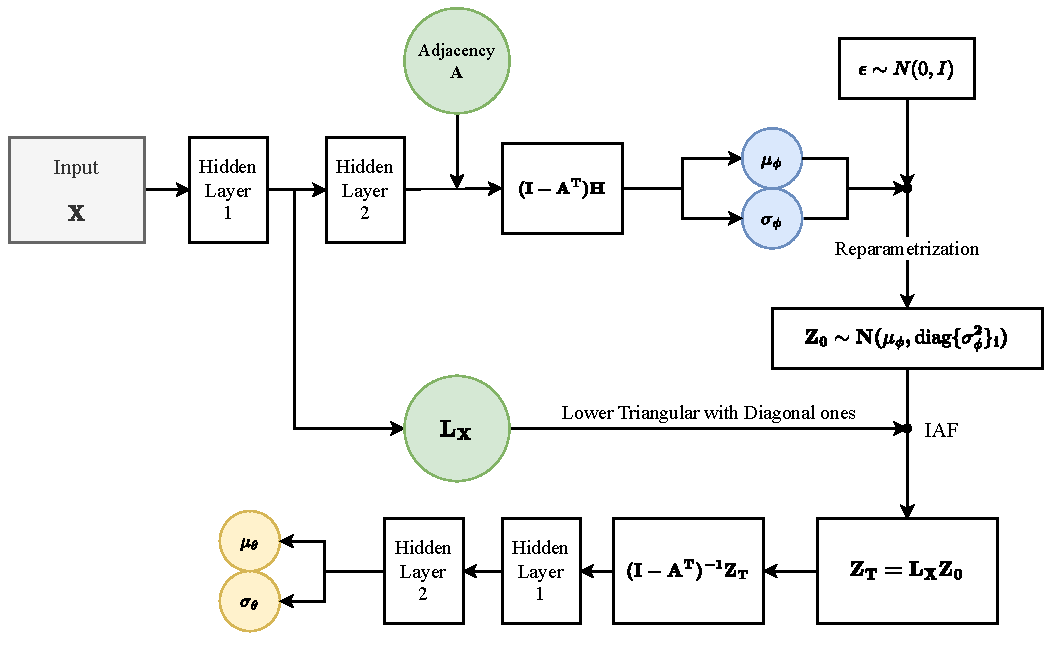
\includegraphics[width=0.8\textwidth]{fig/model.pdf}
        \caption{Overall architecture of our model}
        \label{fig:architecture}
    \end{figure}
\end{frame}

\begin{frame}{Learning}
    \begin{itemize}
        \item We use the same optimization procedure as DAG-GNN \footcite{yu2019daggnn}.
        \item The optimization procedure is minimizing the following loss function:
        \begin{equation}
            \mathcal{L}(A, W, \lambda) =-\mathcal{L}_{\mathrm{ELBO}} + \tau \Vert A \Vert_1 + \lambda h(A) + \frac{c}{2} |h(A)|^2.
        \end{equation}
        \item The second term is the L1 regularization term, which encourages sparsity of the adjacency matrix.
        \item The third and fourth terms are the augmented Lagrangian terms.
        \item Gradually increasing the value of $c$ during the training process results the acyclicity constraint to zero.
    \end{itemize}
\end{frame}
            

\section{Experiment}

\begin{frame}{Experiment}
    \begin{itemize}
        \item We compare our method with the DAG-GNN \footcite{yu2019daggnn} with random graph datasets.
        \item thresholding value of extracting graph as 0.3
        \item Erdős–Rényi random graph with 5000 samples
        \item Node size : 10, 20, 30, and 50 nodes
        \item Noise type : (Independent) Gaussian, Laplace, Exponential and (Dependent) Gaussian
    \end{itemize}
\end{frame}

\begin{frame}{Experiment(Cont'd)}
    \begin{itemize}
        \item We evaluate the performance of our method using two metrics: Structural Hamming Distance (SHD), False Discovery Rate (FDR) with respect to the number of predicted edges.
        \item SHD measures the number of edge additions, deletions, and reversals required to transform the estimated graph into the true graph.
        \item FDR represents the ratio of false positives to the total number of predicted edges.
        \item These metrics are calculated by comparing the estimated graph with the true DAG.
        \item For each combination, we generate at least 5 random graphs and calculate the average metrics.
    \end{itemize}
\end{frame}

\section{Result}

\begin{frame}{Independent Noise}
    \begin{columns}
        \begin{column}{0.5\textwidth}
            \begin{figure}
                \centering
                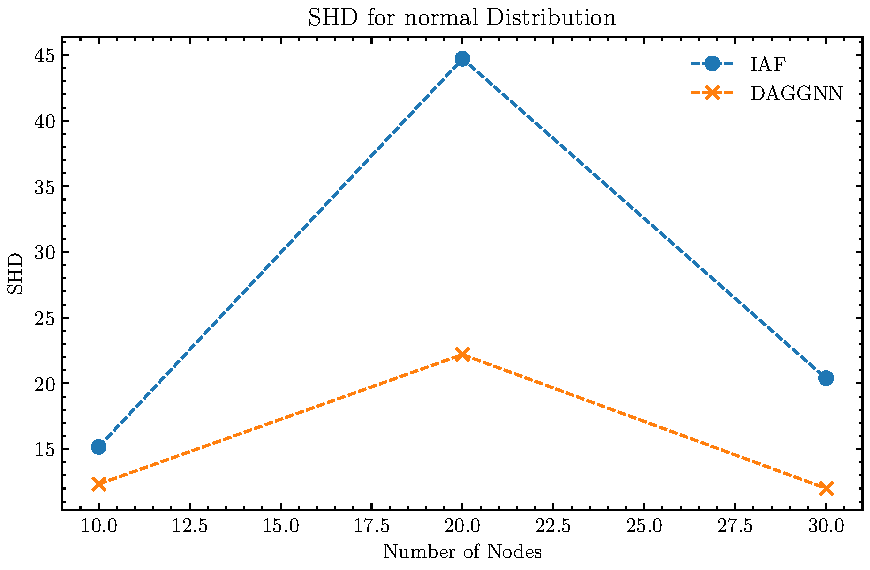
\includegraphics[width=\textwidth]{fig/SHD_independence_normal.pdf}
                \caption{SHD with normal}
                \label{fig:ind_gaussian_shd}
            \end{figure}
        \end{column}
        \begin{column}{0.5\textwidth}
            \begin{figure}
                \centering
                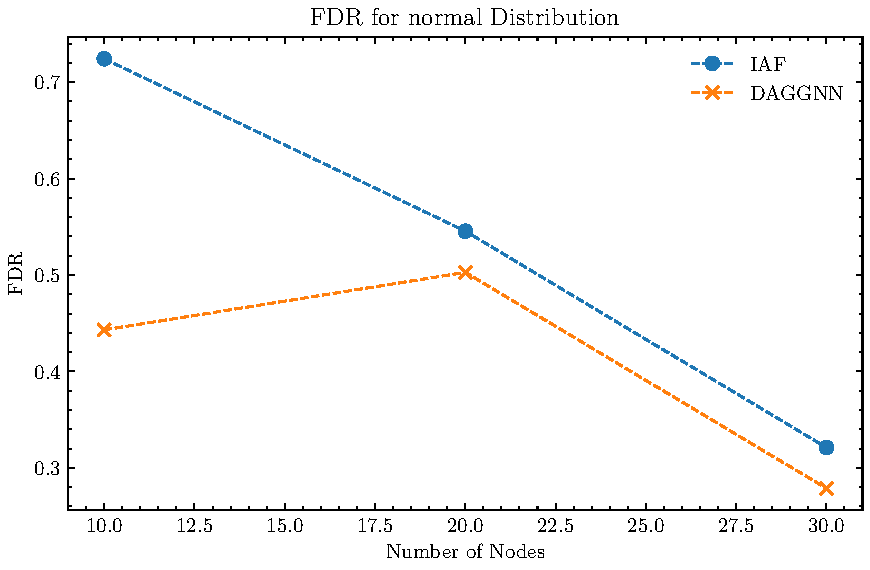
\includegraphics[width=\textwidth]{fig/FDR_independence_normal.pdf}
                \caption{FDR with normal}
                \label{fig:ind_gaussian_fdr}
            \end{figure}
        \end{column}
    \end{columns}
    \begin{itemize}
        \item In the case of independent Gaussian noise, DAG-GNN(orange) performs better than our method(blue).
    \end{itemize}
\end{frame}

\begin{frame}{Independent Noise(Cont'd)}
    \begin{columns}
        \begin{column}{0.5\textwidth}
            \begin{figure}
                \centering
                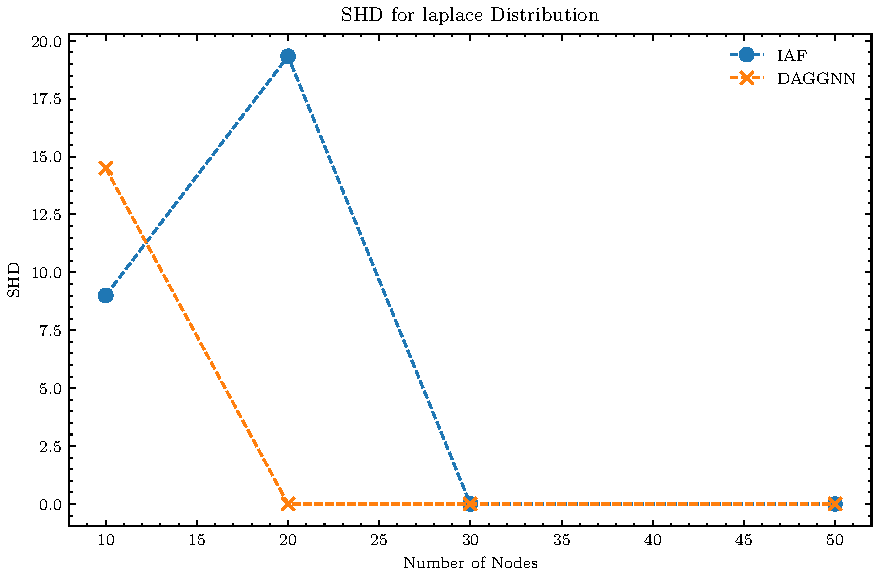
\includegraphics[width=\textwidth]{fig/SHD_independence_laplace.pdf}
                \caption{SHD with Laplace}
                \label{fig:ind_laplace_shd}
            \end{figure}
        \end{column}
        \begin{column}{0.5\textwidth}
            \begin{figure}
                \centering
                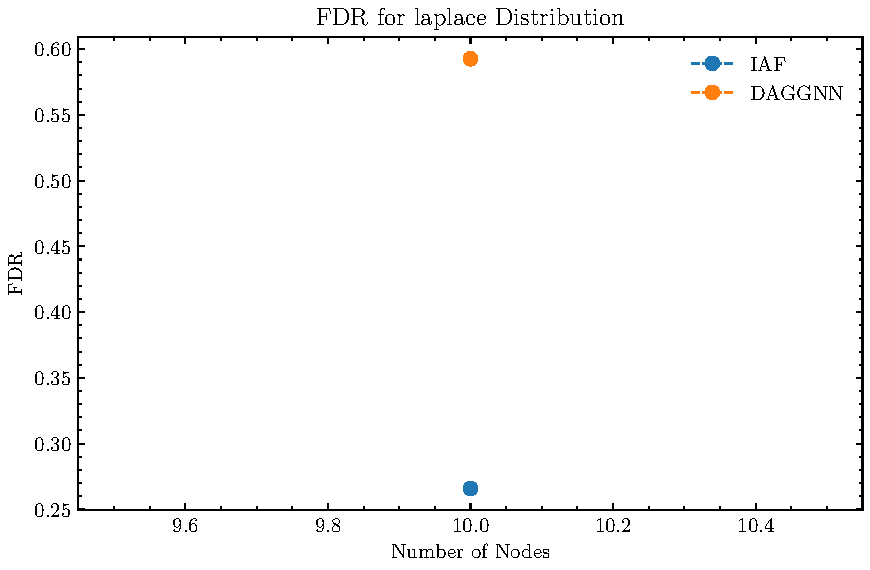
\includegraphics[width=\textwidth]{fig/FDR_independence_laplace.pdf}
                \caption{FDR with Laplace}
                \label{fig:ind_laplace_fdr}
            \end{figure}
        \end{column}
    \end{columns}
    In the case of independent Laplace noise, our method(blue) performs better than DAG-GNN(orange).
\end{frame}

\begin{frame}{Independent Noise(Cont'd)}
    \begin{columns}
        \begin{column}{0.5\textwidth}
            \begin{figure}
                \centering
                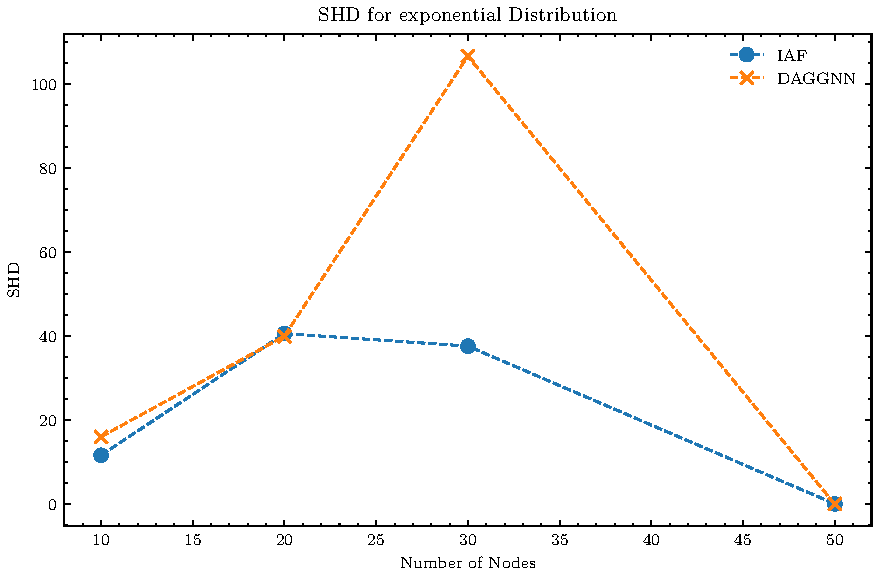
\includegraphics[width=\textwidth]{fig/SHD_independence_exponential.pdf}
                \caption{SHD with Exponential}
                \label{fig:ind_exponential_shd}
            \end{figure}
        \end{column}
        \begin{column}{0.5\textwidth}
            \begin{figure}
                \centering
                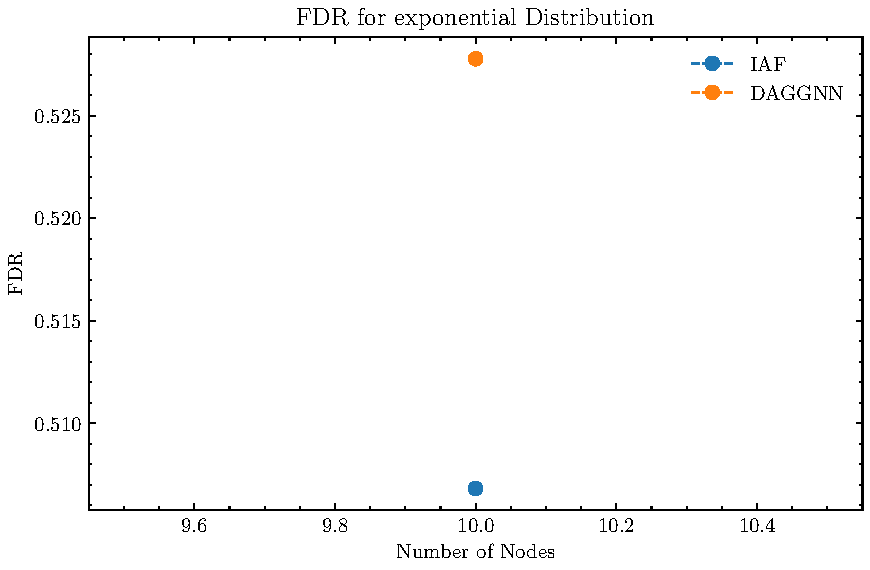
\includegraphics[width=\textwidth]{fig/FDR_independence_exponential.pdf}
                \caption{FDR with Exponential}
                \label{fig:ind_exponential_fdr}
            \end{figure}
        \end{column}
    \end{columns}
    In the case of independent Exponential noise, our method(blue) performs better than DAG-GNN(orange).
\end{frame}

\begin{frame}{Independent Noise(Cont'd)}
    \begin{columns}
        \begin{column}{0.5\textwidth}
            \begin{figure}
                \centering
                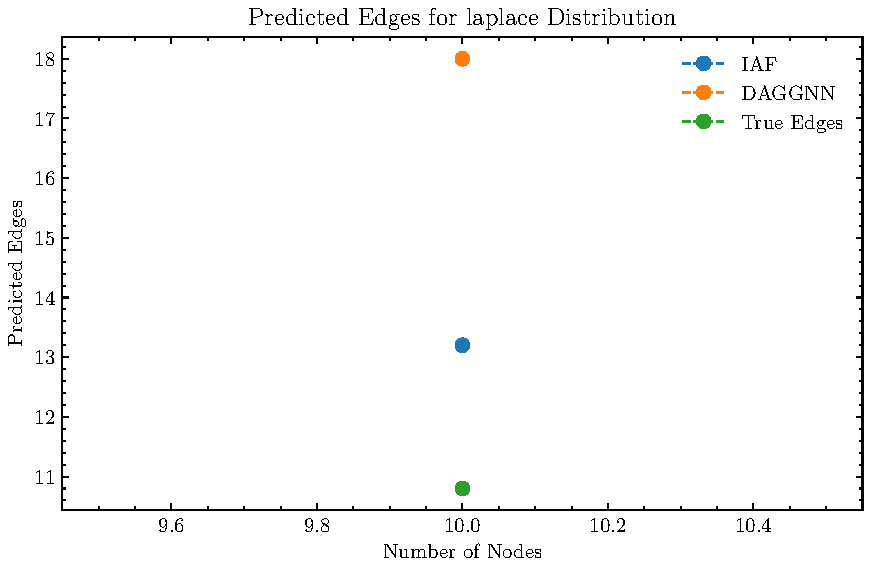
\includegraphics[width=\textwidth]{fig/Predicted Edges_independence_laplace.pdf}
                \caption{Number of predicted edges with Laplace}
                \label{fig:ind_laplace_edges}
            \end{figure}
        \end{column}
        \begin{column}{0.5\textwidth}
            \begin{figure}
                \centering
                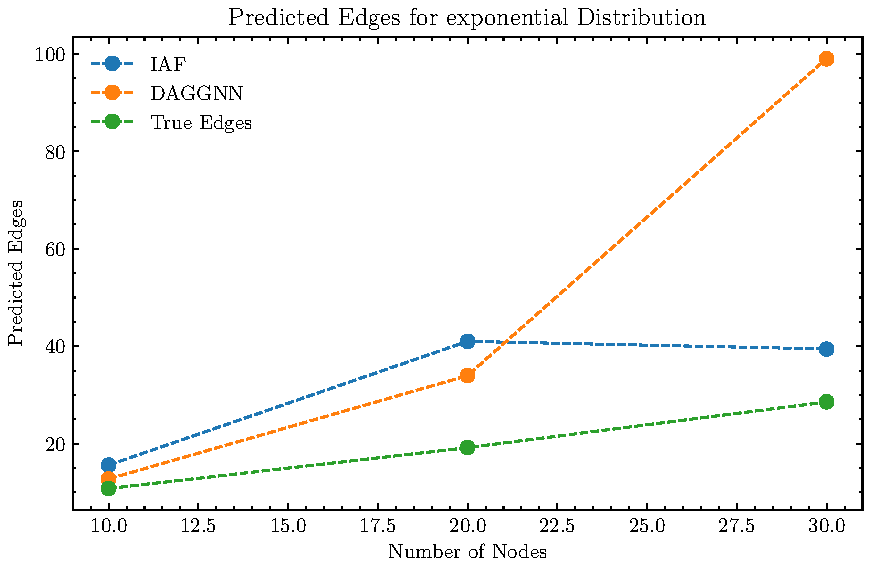
\includegraphics[width=\textwidth]{fig/Predicted Edges_independence_exponential.pdf}
                \caption{Number of predicted edges with Exponential}
                \label{fig:ind_exponential_edges}
            \end{figure}
        \end{column}
    \end{columns}
    Considering the number of predicted edges with the SHD and FDR, our method(blue) performs better than DAG-GNN(orange).
\end{frame}

\begin{frame}
    \begin{figure}
        \centering
        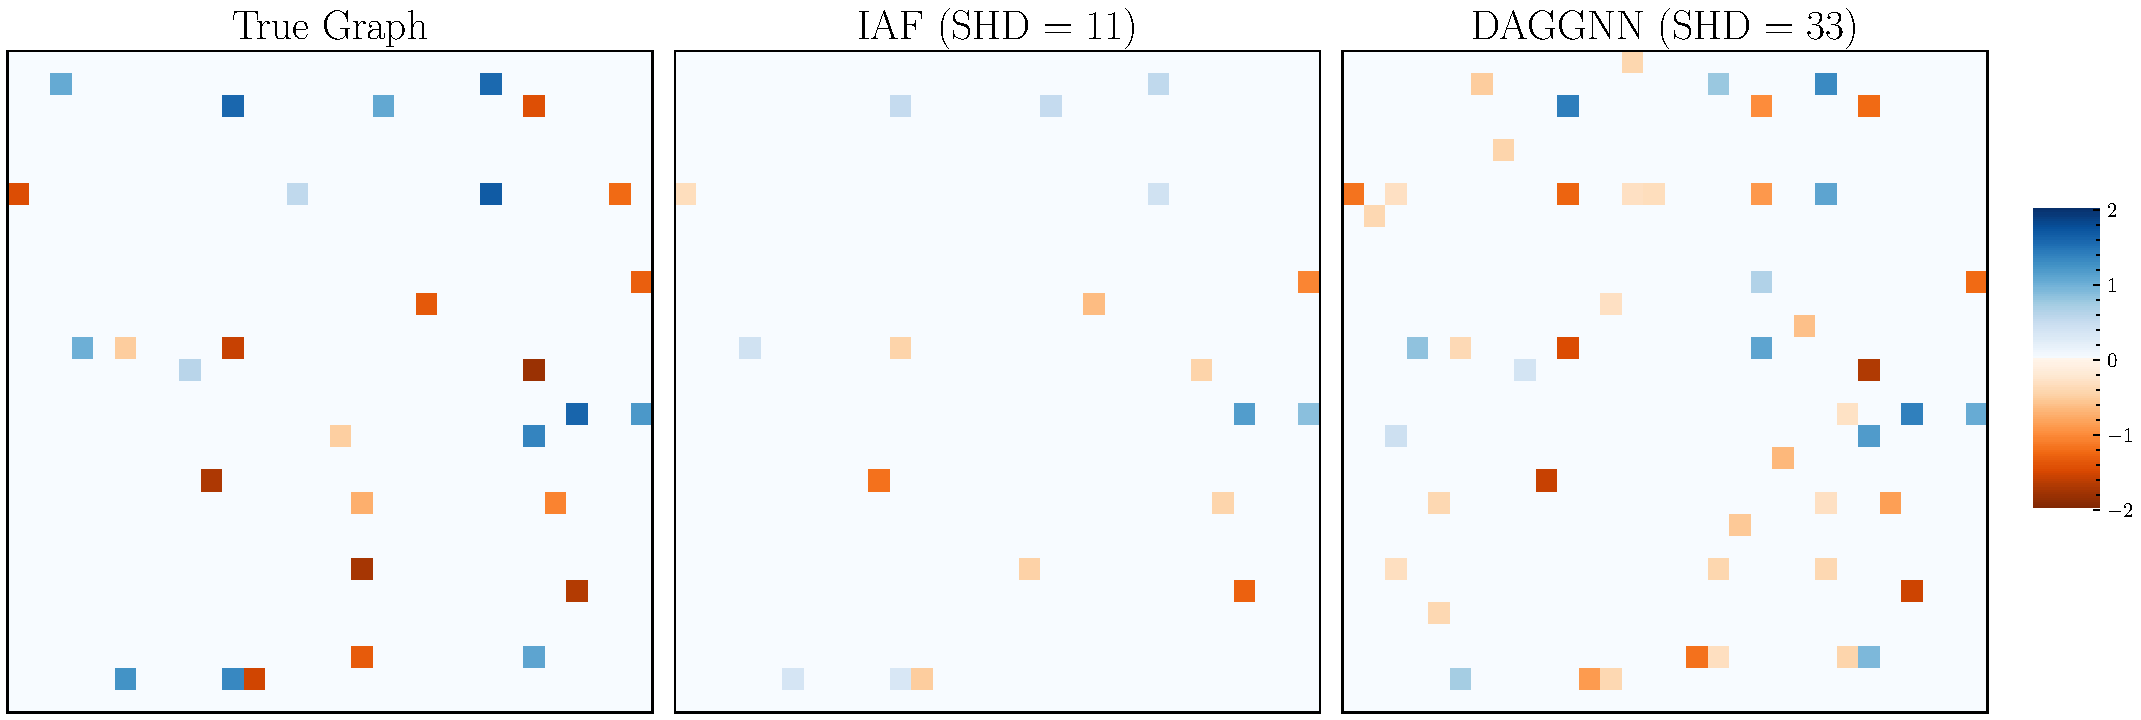
\includegraphics[height=3.5cm]{fig/comparison_indep_30_laplace_seed301.pdf}
        \label{fig:ind_exponential_comparison}
    \end{figure}
    \begin{figure}
        \centering
        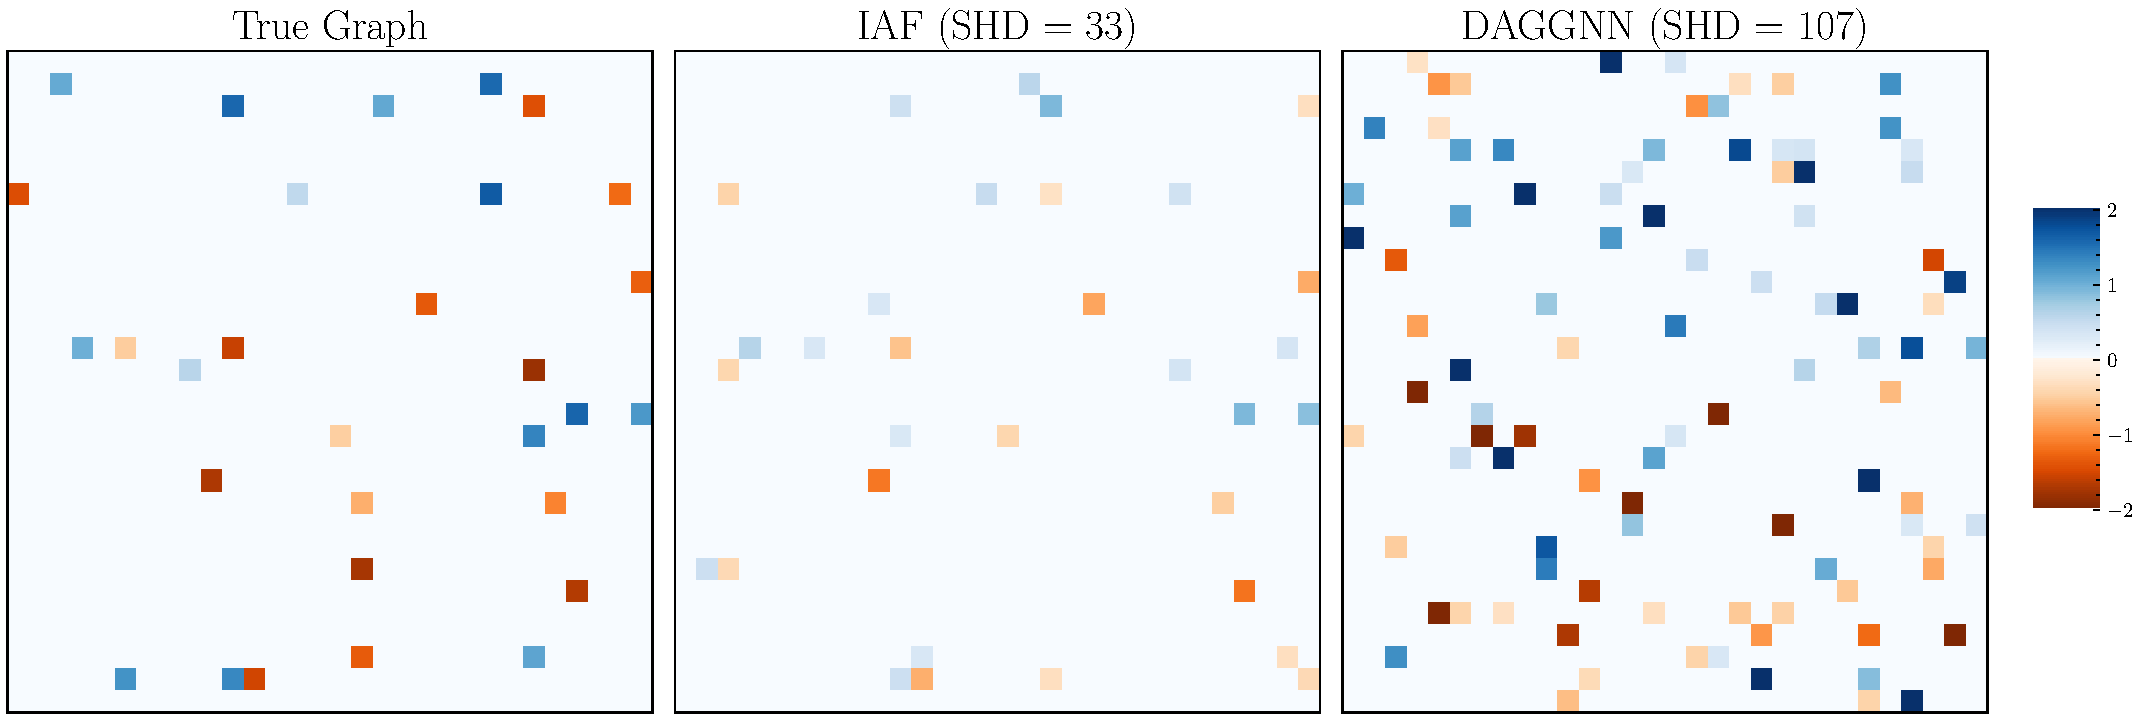
\includegraphics[height=3.5cm]{fig/comparison_indep_30_exponential_seed301.pdf}
        \label{fig:ind_exponential_comparison}
        \captionsetup{justification=centering}
        \caption{Comparison of estimated graphs with Laplace(above) and Exponential(below) noise}
    \end{figure}
\end{frame}

\begin{frame}{Dependent Noise}
    Proportion of bidirectional edges fixed to 0.3.
    \begin{columns}
        \begin{column}{0.5\textwidth}
            \begin{figure}
                \centering
                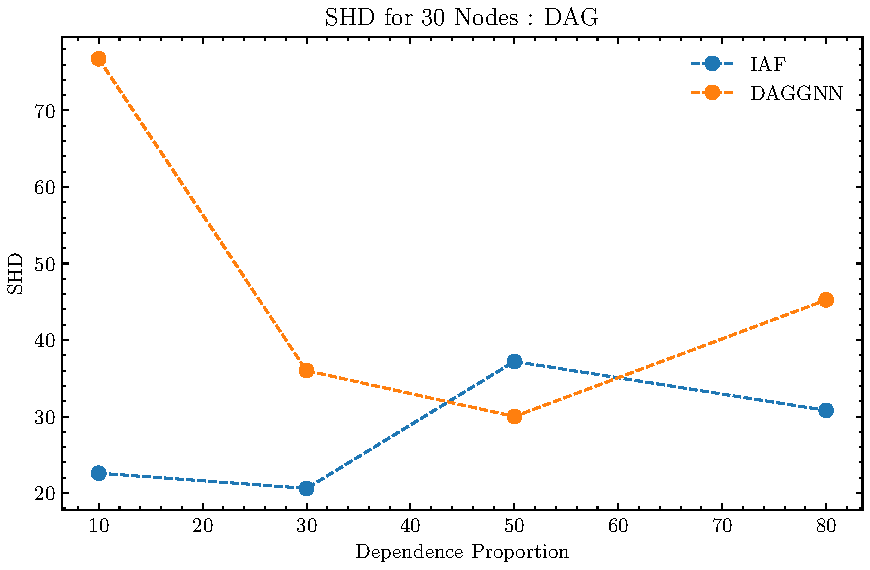
\includegraphics[width=\textwidth]{fig/SHD_dependence_30_DAG_threshold0.3.pdf}
                \caption{SHD with dependent Gaussian}
                \label{fig:dep_gaussian_shd}
            \end{figure}
        \end{column}
        \begin{column}{0.5\textwidth}
            \begin{figure}
                \centering
                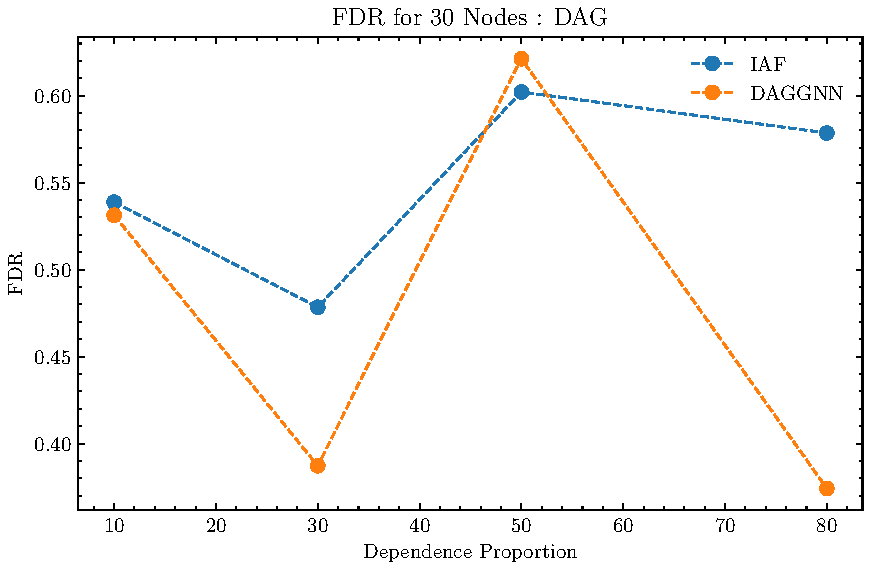
\includegraphics[width=\textwidth]{fig/FDR_dependence_30_DAG_threshold0.3.pdf}
                \caption{FDR with dependent Gaussian}
                \label{fig:dep_gaussian_fdr}
            \end{figure}
        \end{column}
    \end{columns}
\end{frame}

\begin{frame}{Dependent Noise(Cont'd)}
    Proportion of bidirectional edges fixed to 0.3.
    \begin{figure}
        \centering
        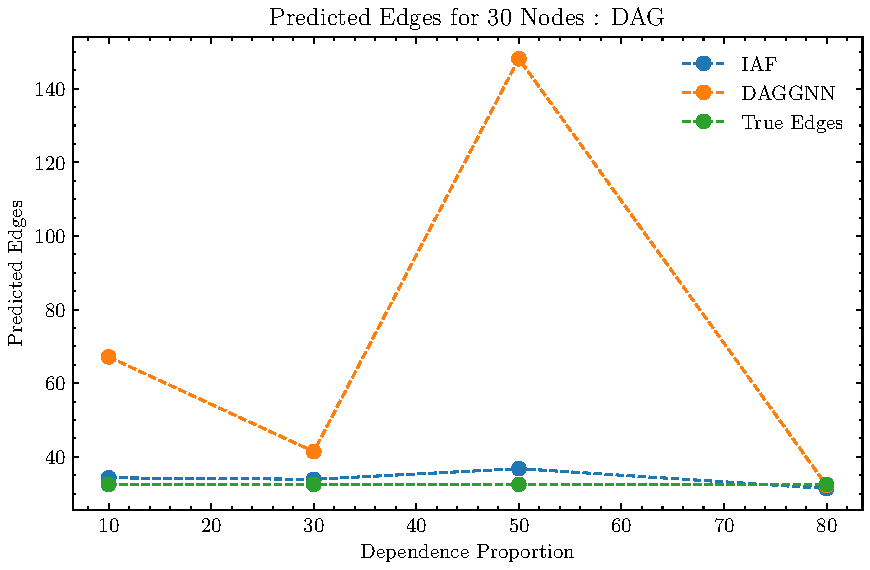
\includegraphics[height=4cm]{fig/Predicted Edges_dependence_30_DAG_threshold0.3.pdf}
        \caption{Number of predicted edges with dependent Gaussian}
        \label{fig:dep_gaussian_edges}
    \end{figure}
    \begin{itemize}
        \item In the case of dependent Gaussian noise, our method(blue) performs better than DAG-GNN(orange).
        \item Considering the stable number of predicted edges with the SHD and FDR, our method(blue) outperforms.
    \end{itemize}
\end{frame}

\begin{frame}{Dependent Noise(Cont'd)}
    Node size $m=10$ : similar performance between DAG-GNN(orange) and our method(blue).
    \begin{columns}
        \begin{column}{0.5\textwidth}
            \begin{figure}
                \centering
                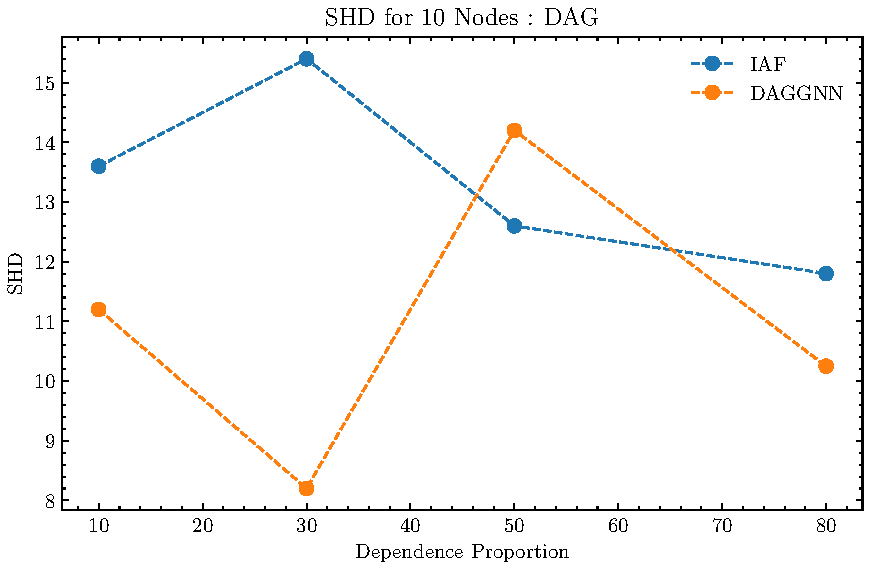
\includegraphics[height=4cm]{fig/SHD_dependence_10_DAG_threshold0.3.pdf}
                \caption{SHD with dependent Gaussian}
                \label{fig:dep_gaussian_shd_10}
            \end{figure}
        \end{column}
        \begin{column}{0.5\textwidth}
            \begin{figure}
                \centering
                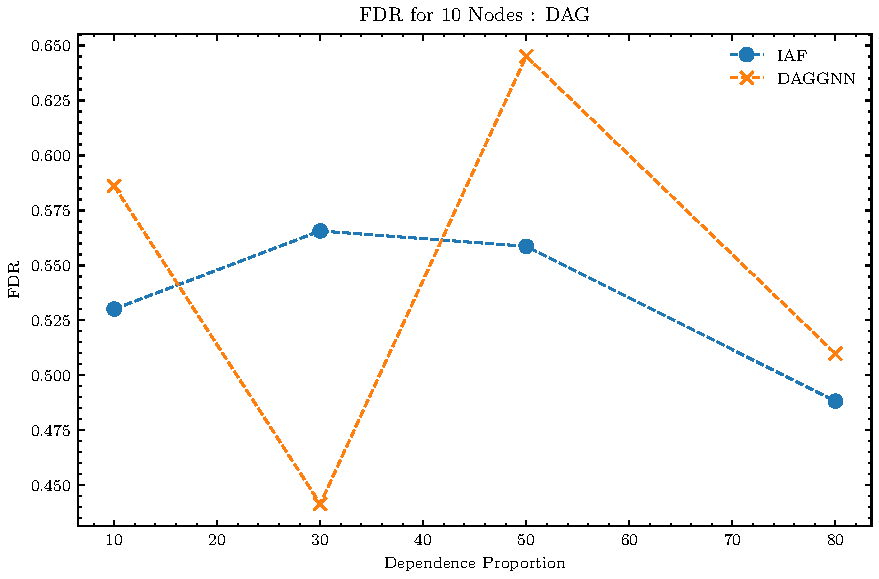
\includegraphics[height=4cm]{fig/FDR_dependence_10_DAG_threshold0.3.pdf}
                \caption{FDR with dependent Gaussian}
                \label{fig:dep_gaussian_fdr_10}
            \end{figure}
        \end{column}
    \end{columns}
\end{frame}

\begin{frame}{Dependent Noise(Cont'd)}
    Node size $m=20$ : our method(blue) performs better than DAG-GNN(orange).
    \begin{columns}
        \begin{column}{0.5\textwidth}
            \begin{figure}
                \centering
                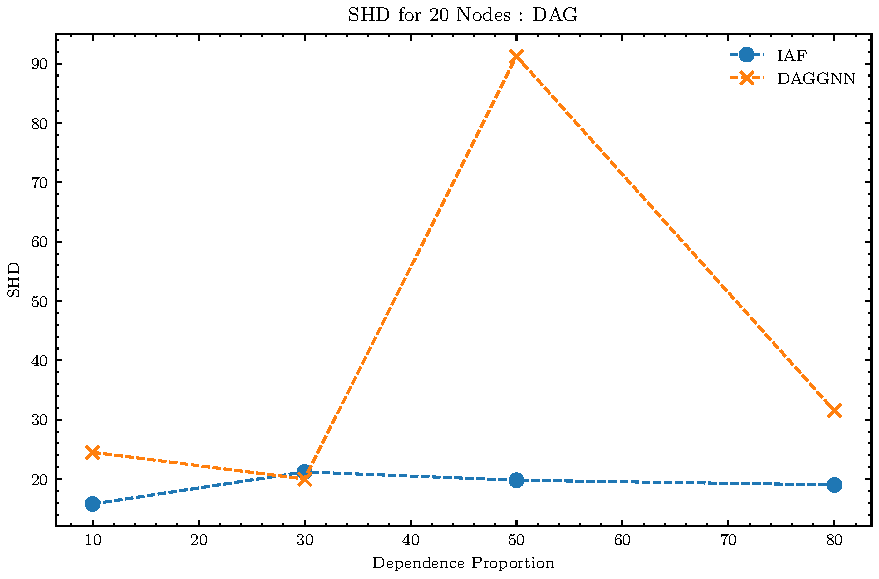
\includegraphics[height=4cm]{fig/SHD_dependence_20_DAG_threshold0.3.pdf}
                \caption{SHD with dependent Gaussian}
                \label{fig:dep_gaussian_shd_20}
            \end{figure}
        \end{column}
        \begin{column}{0.5\textwidth}
            \begin{figure}
                \centering
                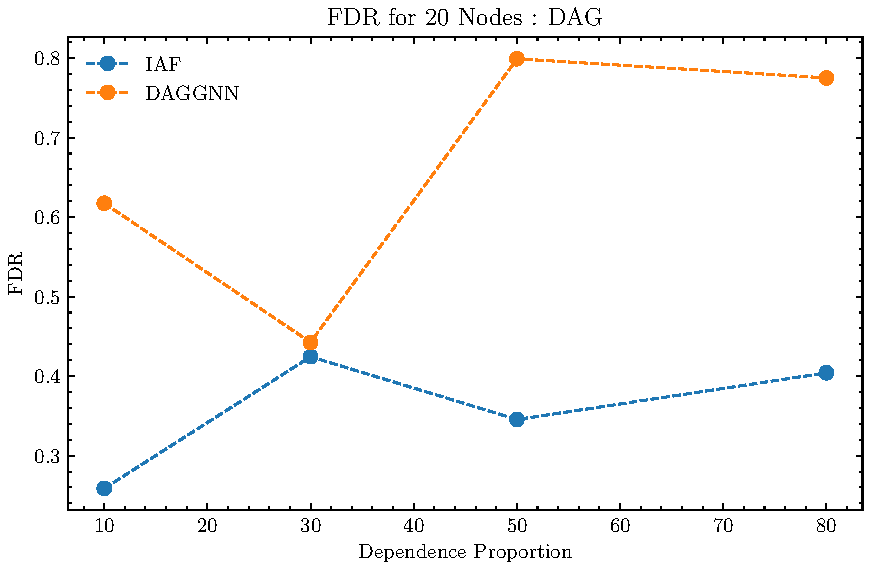
\includegraphics[height=4cm]{fig/FDR_dependence_20_DAG_threshold0.3.pdf}
                \caption{FDR with dependent Gaussian}
                \label{fig:dep_gaussian_fdr_20}
            \end{figure}
        \end{column}
    \end{columns}
\end{frame}

\begin{frame}{Dependent Noise(Cont'd)}
    Node size $m=30$ : our method(blue) performs better than DAG-GNN(orange).
    \begin{columns}
        \begin{column}{0.5\textwidth}
            \begin{figure}
                \centering
                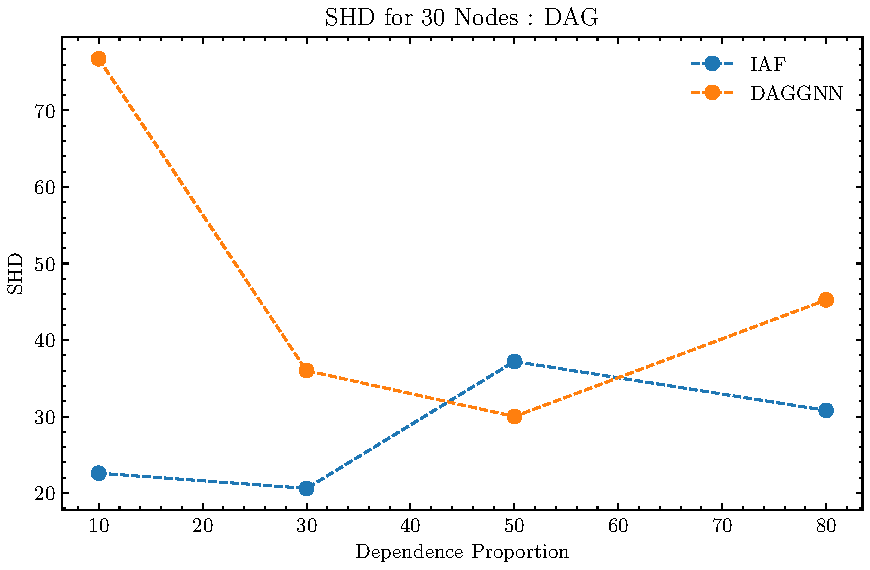
\includegraphics[height=4cm]{fig/SHD_dependence_30_DAG_threshold0.3.pdf}
                \caption{SHD with dependent Gaussian}
                \label{fig:dep_gaussian_shd_30}
            \end{figure}
        \end{column}
        \begin{column}{0.5\textwidth}
            \begin{figure}
                \centering
                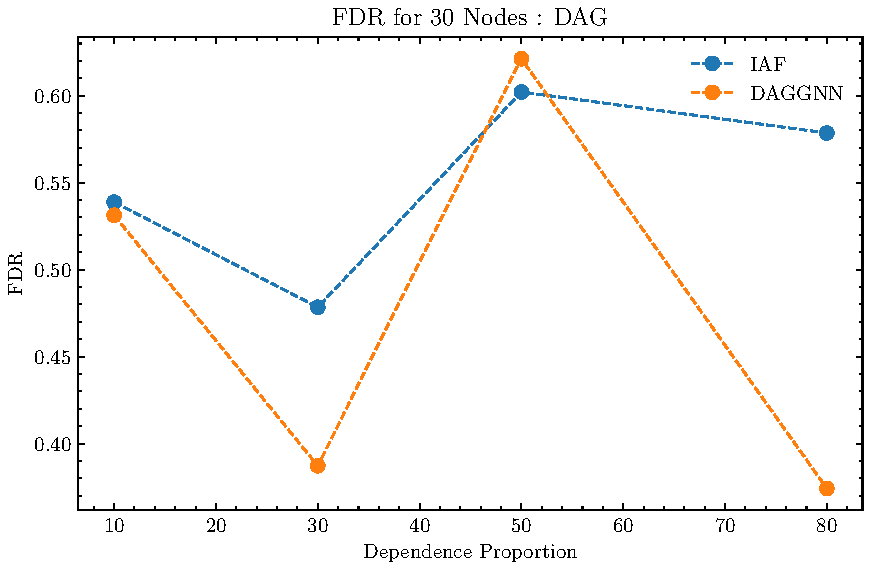
\includegraphics[height=4cm]{fig/FDR_dependence_30_DAG_threshold0.3.pdf}
                \caption{FDR with dependent Gaussian}
                \label{fig:dep_gaussian_fdr_30}
            \end{figure}
        \end{column}
    \end{columns}
\end{frame}

\begin{frame}{Dependent Noise(Cont'd)}
    Node size $m=50$ : our method(blue) performs better than DAG-GNN(orange).
    \begin{columns}
        \begin{column}{0.5\textwidth}
            \begin{figure}
                \centering
                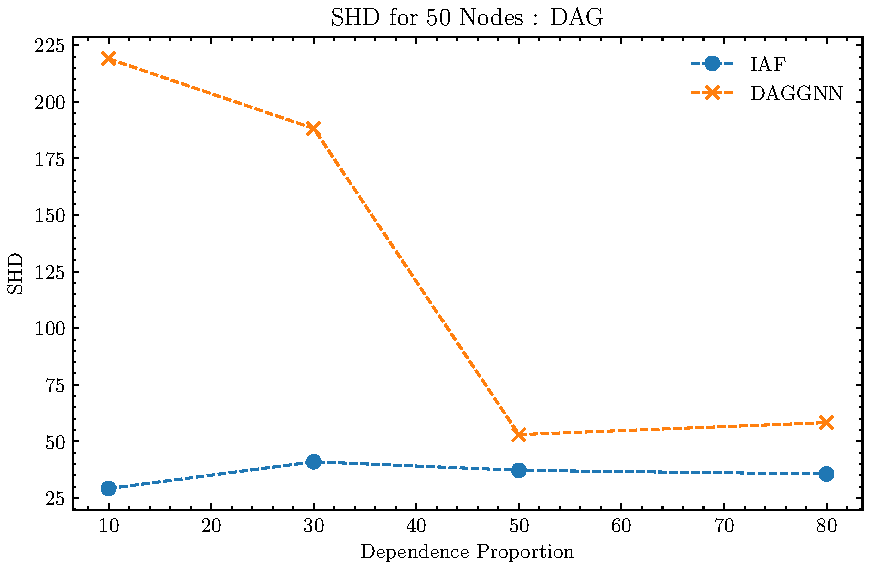
\includegraphics[height=4cm]{fig/SHD_dependence_50_DAG_threshold0.3.pdf}
                \caption{SHD with dependent Gaussian}
                \label{fig:dep_gaussian_shd_50}
            \end{figure}
        \end{column}
        \begin{column}{0.5\textwidth}
            \begin{figure}
                \centering
                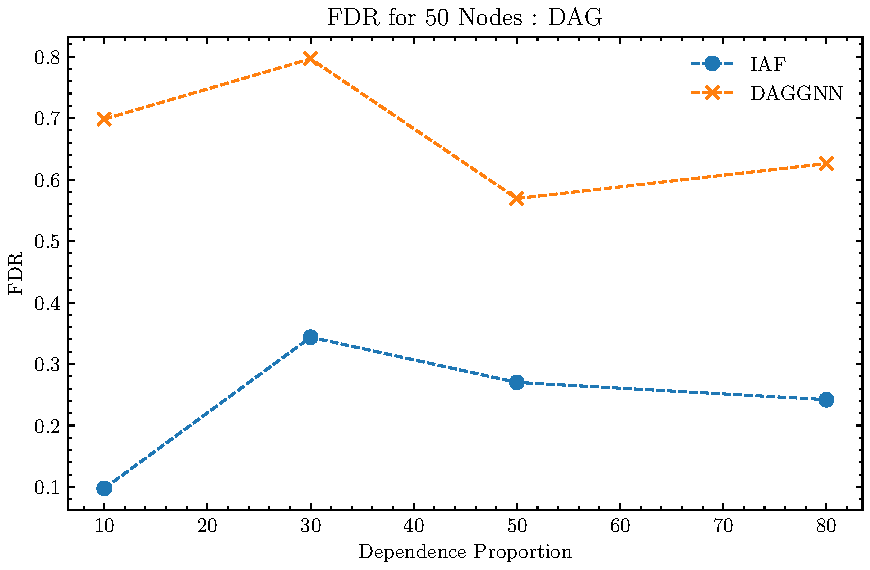
\includegraphics[height=4cm]{fig/FDR_dependence_50_DAG_threshold0.3.pdf}
                \caption{FDR with dependent Gaussian}
                \label{fig:dep_gaussian_fdr_50}
            \end{figure}
        \end{column}
    \end{columns}
\end{frame}

\begin{frame}{Number of predicted edges}
    \begin{columns}
        \begin{column}{0.5\textwidth}
            \begin{figure}
                \centering
                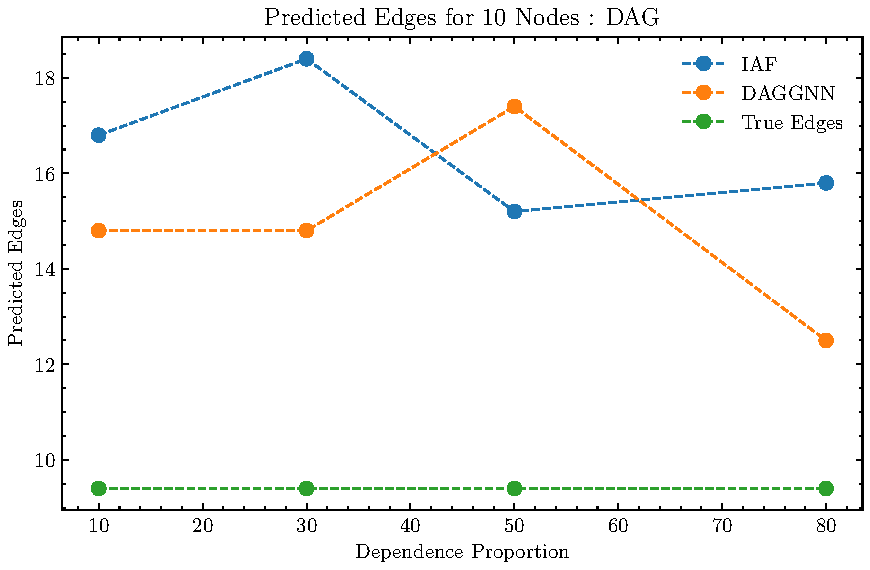
\includegraphics[scale=0.3]{fig/Predicted Edges_dependence_10_DAG_threshold0.3.pdf}
                \caption{$m=10$}
                \label{fig:dep_gaussian_edges_10}
            \end{figure}
        \end{column}
        \begin{column}{0.5\textwidth}
            \begin{figure}
            \centering
            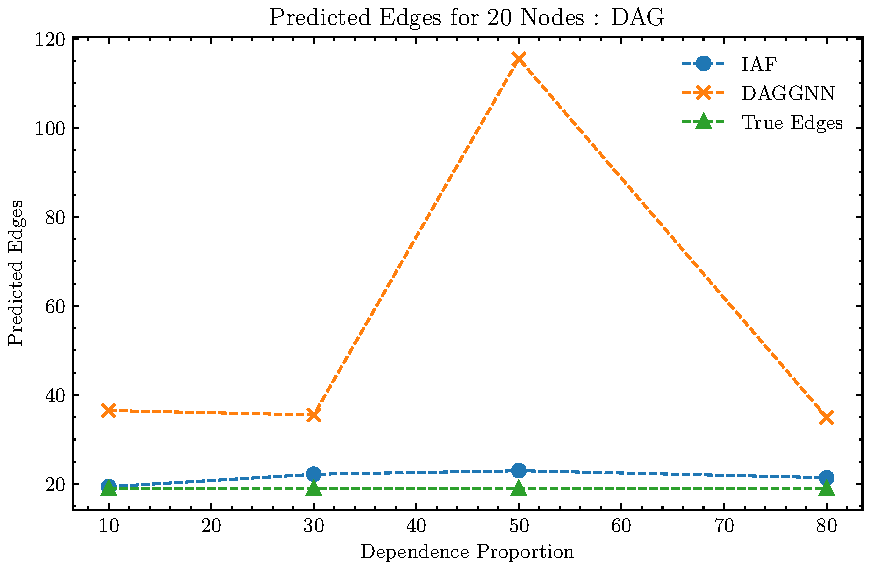
\includegraphics[scale=0.3]{fig/Predicted Edges_dependence_20_DAG_threshold0.3.pdf}
            \caption{$m=20$}
            \label{fig:dep_gaussian_edges_20}
            \end{figure}
        \end{column}
    \end{columns}
    \begin{columns}
        \begin{column}{0.5\textwidth}
        \begin{figure}
            \centering
            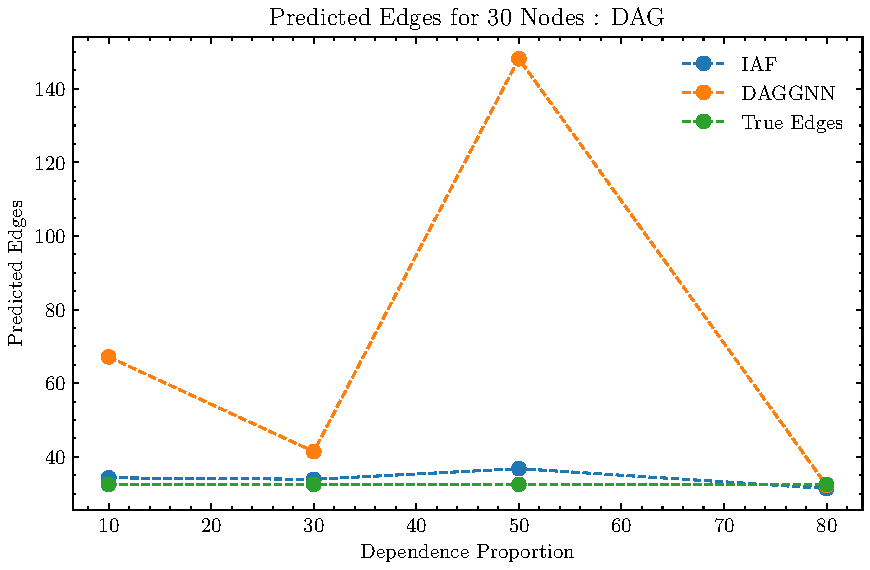
\includegraphics[scale=0.3]{fig/Predicted Edges_dependence_30_DAG_threshold0.3.pdf}
            \caption{$m=30$}
            \label{fig:dep_gaussian_edges_30}
        \end{figure}
        \end{column}
        \begin{column}{0.5\textwidth}
        \begin{figure}
            \centering
            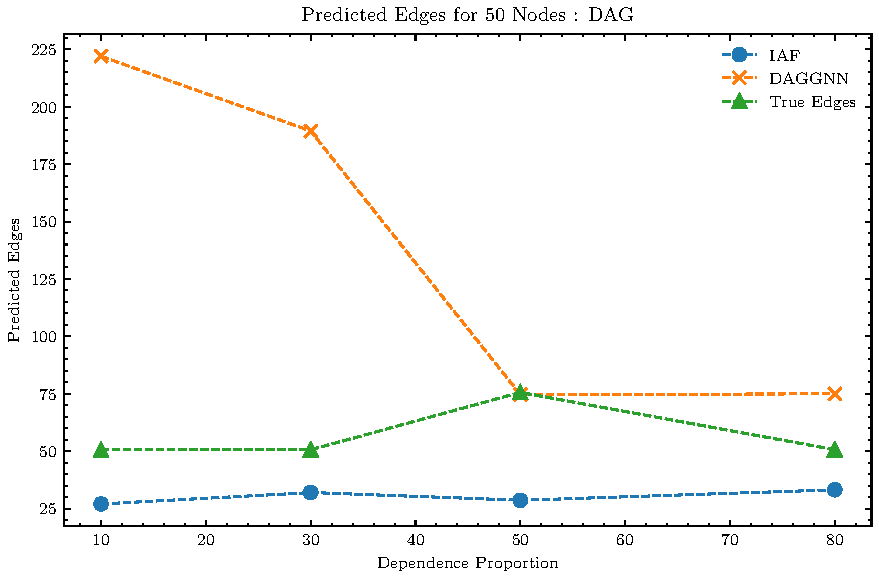
\includegraphics[scale=0.3]{fig/Predicted Edges_dependence_50_DAG_threshold0.3.pdf}
            \caption{$m=50$}
            \label{fig:dep_gaussian_edges_50}
        \end{figure}
        \end{column}
    \end{columns}    
\end{frame}

\section{Conclusion}

\begin{frame}{Conclusion}
    \begin{itemize}
        \item Proposed a method to learn the structure of a semi-Markovian DAG using a flow-based VAE.
        \item Conducted experiments on simulated data and compared the performance of our method with that of DAG-GNN.
        \item Our method outperforms DAG-GNN in terms of both SHD and FDR metrics, especially when the noise variables have a dependent structure and when the size of the graph is large.
        \item In terms of the number of predicted edges, our method results in fewer edges than DAG-GNN while maintaining the same or better level of SHD and FDR. 
    \end{itemize}
\end{frame}

\begin{frame}{Conclusion(Cont'd)}
    \begin{itemize}
        \item However, contrary to our initial expectations, the lower triangular matrix $\mathbf L$ learned in the IAF layer did not capture the covariance matrix of the actual noise variables.
        \item This seems to be due to the entanglement problem in the latent space, and resolving this issue remains a future research task.
        \item If the full covariance matrix of the noise variables could be found, it could be possible to directly identify bidirectional edges in the graph, enabling more accurate learning of the semi-Markovian graph.
    \end{itemize} 
\end{frame}





\begin{frame}[allowframebreaks]{References}
\printbibliography
\end{frame}
\end{document}